% !TeX spellcheck = en_EN-English

\section{Future record prediction}
\label{record_prediction}

This task is most important while also hardest to train. Our goal is to create model which would be able to predict potential next record based on patient previous ones. This task in general is almost impossible with amount of information we have, since there are many other factors that determine whether, when and what new disease will the patient become infected with in the future, whether his current state will improve or worsen, and most importantly what specific steps will doctor take.
\\

Fortunately our ultimate goal is not to predict specific patient future but only estimate how much would he most likely cost. So we expect that even though we wouldn't predict what exactly happens we would be able to estimate total cost of those records.
\\

We try multiple different model for this prediction. First three models we tried were recurrent neural networks (RNN). More specifically we tried multi-layer Elman RNN, multi-layered gated recurrent unit (GRU) RNN and multi-layer long short-term memory (LSTM) RNN. Last model we tried was Transformer.
\\

\subsection{Recurrent neural network}

In general recurrent neural network is type of neural network that in some way uses results from previous step or steps in order to improve prediction. These models are used for ordered data where next step is dependent on more than single previous one.

\subsection{Elman RNN}

Elman RNN also known as simple recurrent network (SNR) is type of recurrent neural network that utilize results of hidden layer before activation in previous step as an additional input in next one. We can see this architecture on figure \ref{fig:elman_arch}, where on left we can see how forward propagation look and on right how it looked unrolled over time, we see that middle layer which is a hidden layer of model gets two inputs, first is input vector $x_t$, where $t$ denotes step (usually time step), which is multiplied with matrix of weights $W_i$ and second one is vector $h_{t-1}$ which is result of this layer also called context vector in previous step. which is multiplied by different matrix of weight denoted as $W$, these two results after they are then summed together and result goes to activation layer which create resulting new vector $h_t$ \cite{elman}, this whole process can be summarized by this equation (where $b_i$ and $b$ are bias vectors):

\begin{equation}
	\label{eqn:elman}
	h_t = act(x_t W^T_i + b_i + h_{t-1} W^T + b)
\end{equation} 

Usually this result is directly used as output or go into single fully-connected feed-forward layer. In multi-layered version of this network, result of first hidden layer would go into next hidden layer together with result of that specific layer in previous step and again both would get multiplied by matrices of weight specific for that layer, summed and results goes through activation function.
\\

\begin{figure}[!h]
	\centering
	
	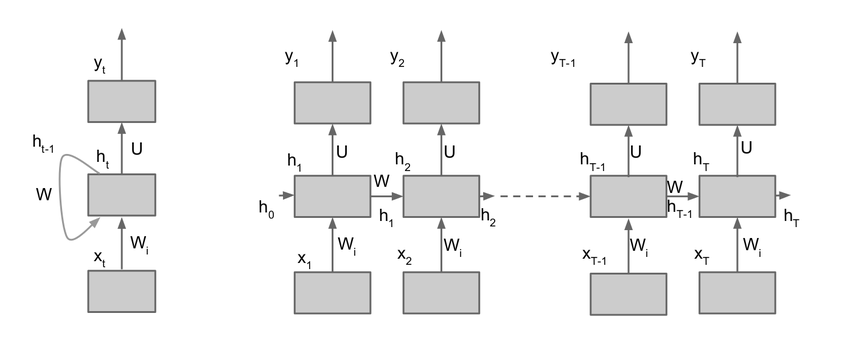
\includegraphics[width=0.85\textwidth]{images/Elman_RNN_architecture.png}
	
	\caption{Architecture of Elman RNN \cite{elman_img}}
	\label{fig:elman_arch}
\end{figure}

  

\subsection{Gated recurrent unit}
 
Gated recurrent unit is more complex recurrent neural network compared to Elman RNN. This model was developed as simplification of even more complex LSTM model. We can say that it consist mainly of three parts that interact with each other and together create final prediction. Those parts are reset gate, update gate and candidate hidden state computation. We can see structure of hidden layer of GRU on figure \ref{fig:gru_arch}. On this diagram sigmoid means fully-connected feed-forward layer with sigmoid activation function and tanh means fully-connected feed-forward layer with hyperbolic tangent activation function.
\\

Reset gate is on left side of diagram, it's task is to using input and previous hidden state vectors modify previous hidden state vector which goes into candidate hidden state computation. This should helps capture short-term dependencies in time series.
\\

Candidate hidden vector computation is part that is similar to Elman RNN with two differences, firstly inputted hidden layer is modified by reset gate result and secondly resulting vector from this part is only candidate which goes into further calculation
\\

Update gate, similarly to reset gate, uses concatenation of input and previous hidden state vector on input, but this time results are used to modify both previous hidden state and candidate hidden state in a way that resulting hidden state is weighted average of those two vectors where weights are results from this gate. This should help to capture long-term dependencies in time series. 
\\ 

\begin{figure}[!h]
	\centering
	
	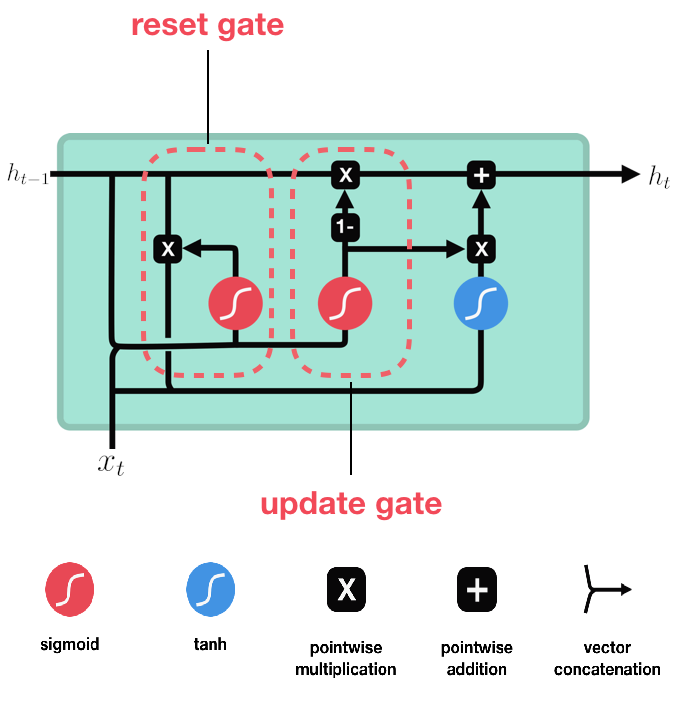
\includegraphics[width=0.6\textwidth]{images/GRU_arch.png}
	
	\caption{Architecture of GRU hidden layer}
	\label{fig:gru_arch}
\end{figure}
 
Multi-layered version is achieved by stacking hidden layers where hidden state vector of one layer is input vector of next one.
 
\subsection{Long short-term memory}

As mentioned earlier, long short-term memory is more complex predecessor of GRU. This model was developed with aim to mitigate vanishing gradient problem, that cause lack of long-term memory in models like Elman RNN, mainly by introducing memory vector that should maintain information over longer period. As we can see in figure \ref{fig:lstm_arch} this model consist of three gates, candidate memory computation. 

 
\begin{figure}[!h]
	\centering
 	
	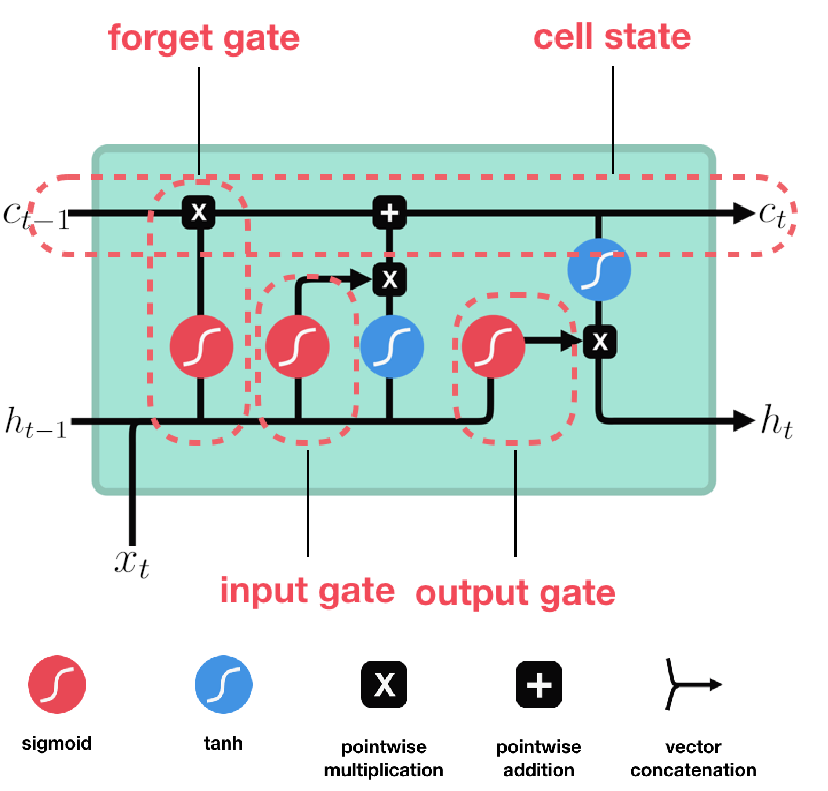
\includegraphics[width=0.6\textwidth]{images/LSTM_arch.png}
 	
 	\caption{Architecture of LSTM hidden layer}
 	\label{fig:lstm_arch}
\end{figure}